\documentclass[11pt]{amsart}

% Standard letter size paper with 1inch margins
\usepackage[letterpaper, margin=1in]{geometry}

% Useful packages 
\usepackage{amsmath, amssymb, amsthm, amsaddr}
\usepackage{enumerate, subcaption, graphicx, hyperref}


\title{AMATH 482/582: Home Work 1}
\author{Future Scientist} % first and last name

\address{Amazing Department, University of Washington, Seattle, WA 
\\ \texttt{youremail@uw.edu}}

\date{\today} % you can also just type the date instead of "\today"

\begin{document}

\maketitle 

\begin{abstract}
    Your report should contain a brief, 100 word abstract describing what is contained in 
    the document and what you did. {\bf Don't forget 6 pages max}.
\end{abstract}


\section{Introduction and Overview}\label{sec:Introduction}

Here you will give a brief introduction to the problem you solved. Including 
some discussion of relevant literature and background. 

Make sure you use the correct citation commands (i.e., \texttt{$\backslash$cite}) to keys 
from your bib file like this \cite{example-article-citation}. If you want 
to cite more than one reference simply use \cite{example-article-citation, example-book-citation}. You can grab latex citations 
from \href{https://scholar.google.com}{Google Scholar}. Just keep in mind that they often 
need to be cleaned up.

\section{Theoretical Background}\label{sec:theory}

You dedicate this section to the theoretical background of the methods and frameworks 
that you used in your homework. This is not meant to reproduce material from the lectures
 or references you used but rather to demonstrate your understanding of the 
 mathematical foundations of the methods and algorithms. You can create equations like this 
 \begin{equation*}
     f(x) = \int_A \sin( \pi x) dx.
 \end{equation*}
 You do not need to label your equations unless they are referenced in the text. In that 
 case simply use 
 \begin{equation}\label{eq:meaningful-label}
      - \frac{\partial^2 u}{\partial x^2} = \sin ( \pi x).
 \end{equation}
Also look up the \texttt{align} or \texttt{aligned} environments if you want multi-line 
equations. You can then reference your equations in text using the $\backslash$\texttt{eqref}
command as such \eqref{eq:meaningful-label}. 

\section{Algorithm Implementation and Development}\label{sec:algorithms}
Here you discuss the algorithms and software packages that you used. Not much to it. 
Just make sure you cite the packages properly and avoid including code. 
You are welcome to use \LaTeX packages that are specifically designed to show 
algorithms such \href{https://www.overleaf.com/learn/latex/Algorithms}{as this}, but it is 
not always worth the effort and real estate. 


\section{Computational Results}\label{sec:results}

This is perhaps the most important section of your report. You want to dedicate more space 
here and present your numerical results in a clear, concise and meaningful way. Also 
include a discussion of your numerics. Think hard about how you can use 
your space most efficiently. For example, include subplots and multiple error curves on the 
same plot etc. Ask us for advice when the time comes. 

You will most definitely need tables and figures. So here is an example. 

\begin{table}[htp]
    \centering
    \begin{tabular}{| l | c|c | r |}
         \hline
         row 1 & column 1  & column 2  \\ \hline
         row 2 & column 1 & column 2 \\ 
         row 3 & column 1 & column 2 \\ \hline
    \end{tabular}
    \caption{Don't forget to include a caption for your table. Say a few words about what is 
    being shown.}
    \label{tab:meaningful-label}
\end{table}

Make sure your table is labeled and referenced withing the text using $\backslash$\texttt{ref} as such Table~\ref{tab:meaningful-label}. In fact, you can 
use $\backslash$\texttt{ref} to cite anything else in the document such as 
sections (ex. Section~\ref{sec:Introduction}). This will create hyperlinks in your 
pdf after compilation and automatically update the numbers and tags whenever you change 
anything. 

Figures are very similar to tables. Here's an example: 

\begin{figure}[htp]
    \centering
    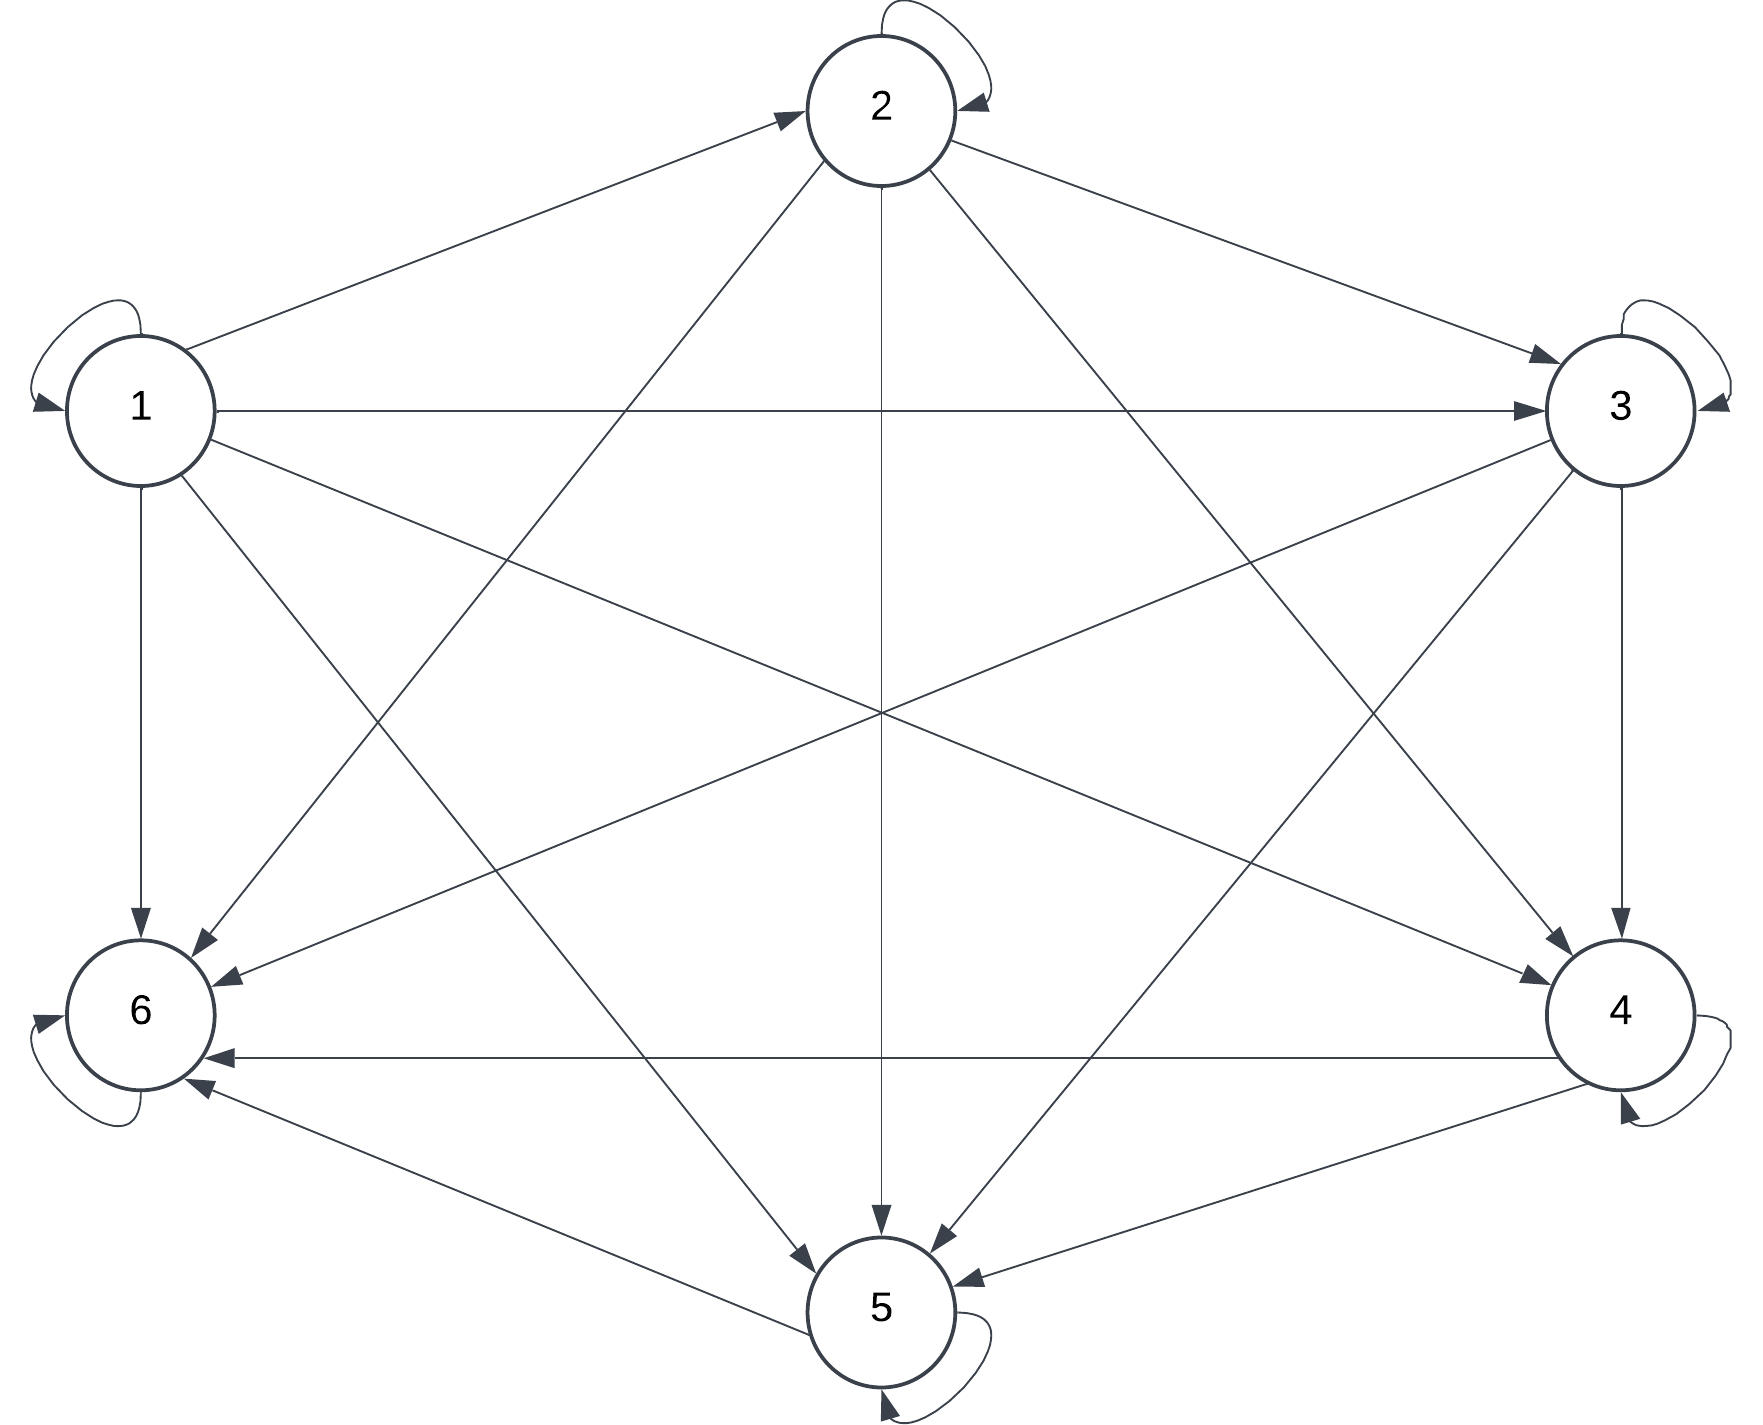
\includegraphics[width=0.4\textwidth]{./Figs/fig1.png}
    \caption{Include a descriptive caption for your figure. Also make sure all 
    legends, axis labels, and titles are large enough to be readable. You might have 
    to reproduce the plots from Python or MATLAB with larger fonts for this purpose. It 
    can be annoying the first time you do it but it is crucial.}
    \label{fig:meaningful-label}
\end{figure}


You may also need to include multiple figures: 

\begin{figure}
    \centering
    \begin{subfigure}[b]{.3\textwidth}
    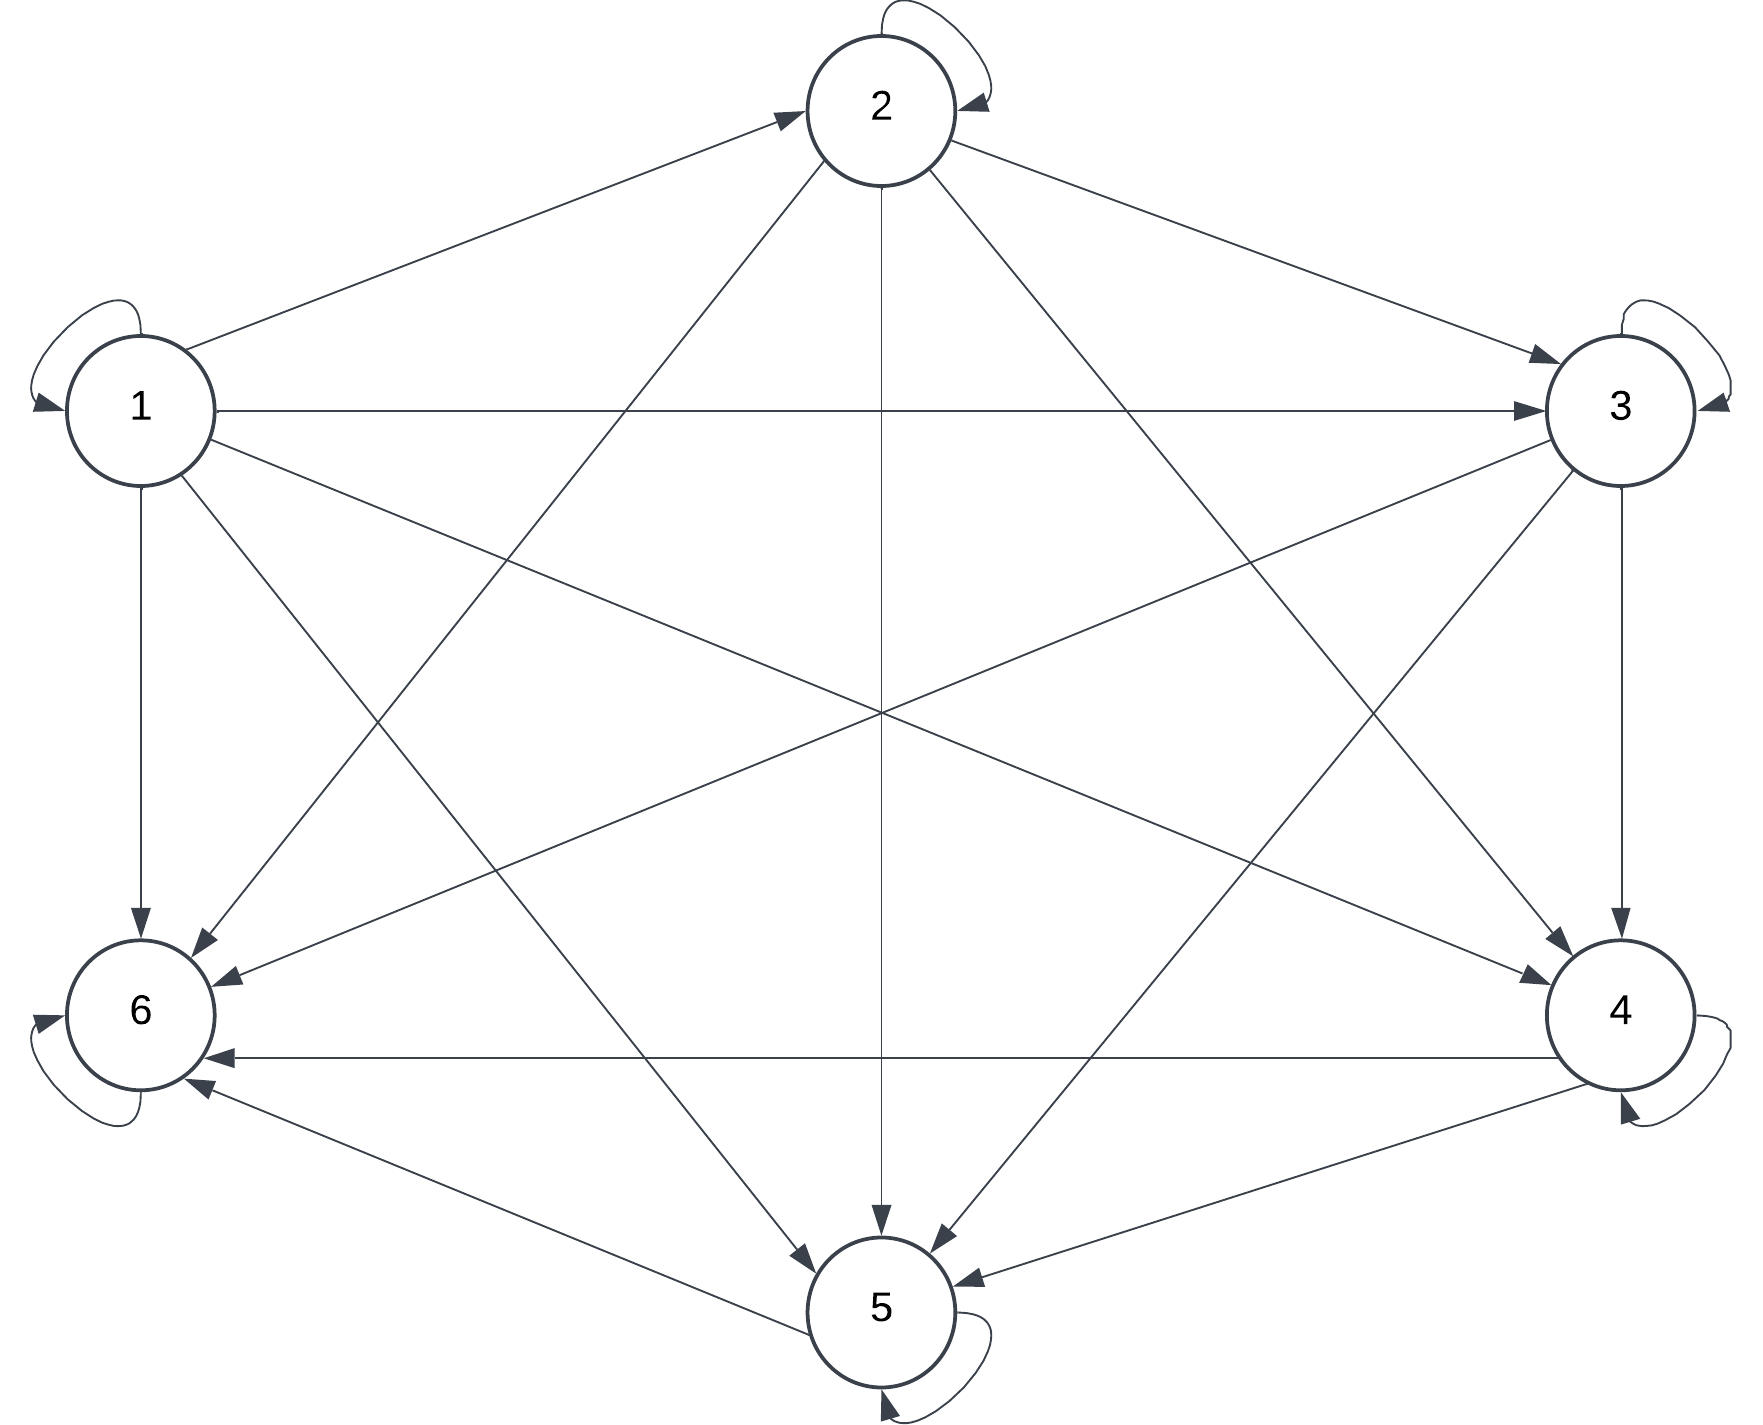
\includegraphics[width=\textwidth]{./Figs/fig1.png}
    \caption{First subfigure}
    \label{subfig:first}
    \end{subfigure}
    \begin{subfigure}[b]{.3\textwidth}
    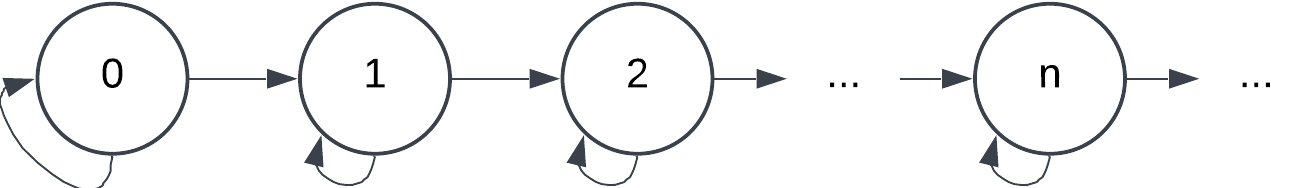
\includegraphics[width=\textwidth]{./Figs/fig2.png}
    \caption{First subfigure}
    \label{subfig:second}
    \end{subfigure}
    \begin{subfigure}[b]{.3\textwidth}
    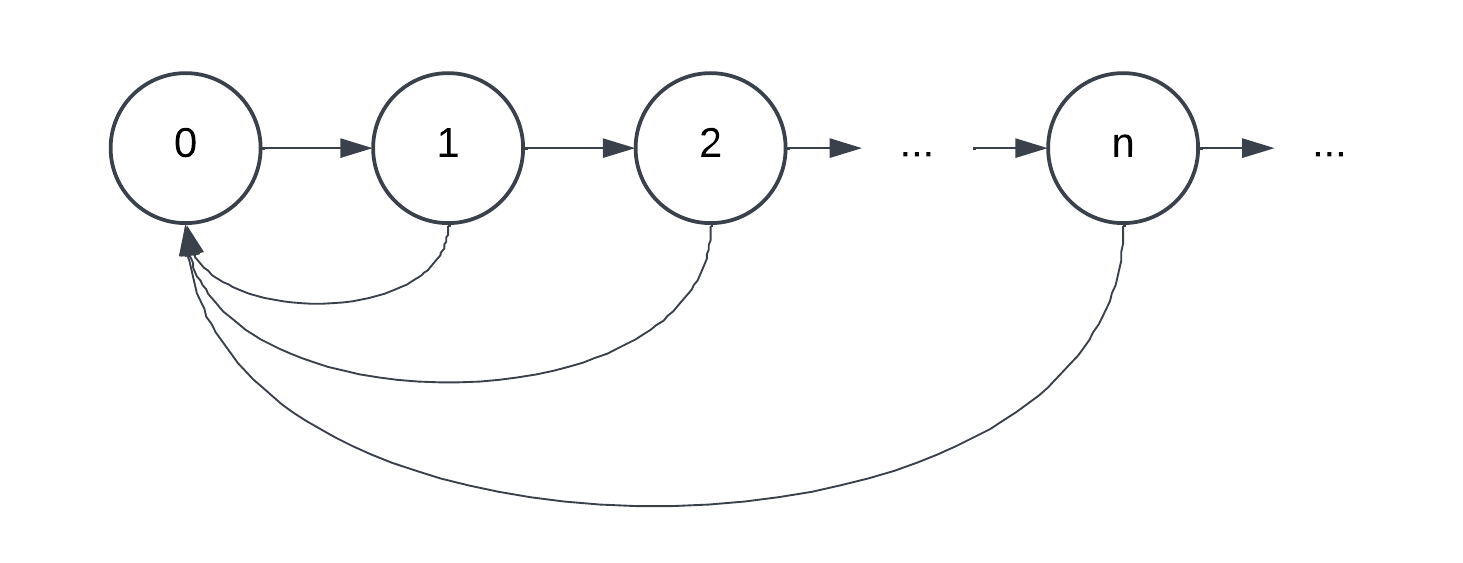
\includegraphics[width=\textwidth]{./Figs/fig3.png}
    \caption{First subfigure}
    \label{subfig:third}
    \end{subfigure}
    \caption{Caption for entire figure. You don't need to use captions for subfigs so 
    feel free to eliminate the subcaption texts to just have the A, B, C labels.}
    \label{fig:meaningful-label-2}
\end{figure}

Once again, make sure all your figures are referenced like Figure~\ref{fig:meaningful-label}
or Figure~\ref{subfig:first} in the text body of the report and discussed 
in detail. This is where you will make observations about your results and we will 
look at these very closely. 

Also note, I am using PDF figures. These give you the best looking graphs but PNG works 
well too. I advise staying away from JPG as it always looks weird and low quality.]
Both Python and MATLAB can output figures in PDF or PNG.

\section{Summary and Conclusions}\label{sec:conclusions}
Wrap up your report with a brief summary of what you did and what you discovered. 
Finish with some conclusions and possibly future directions if any. 

\section*{Acknowledgements}

Make sure you you clearly state any help you received including collaborations 
with your peers. Help from TAs or other mentors, professors, etc that helped you 
with your assignment. Here's a formal example: 

The author is thankful to Prof. X for useful discussions about the QR algorithm. 
We are also thankful to Dr. Strange for suggesting the JAX software package for 
automatic differentiation. Furthermore, our peer Jean Grey was helpful in 
implementation of spectral clustering in Python.

\bibliographystyle{abbrv}
\bibliography{HW_references} % make sure this matches the .bib file for your corresponding document. You also have to maintain your references in the .bib file 

\end{document}
